\subsection{小原型机测试}

\subsubsection{超净室测试}

在STAR的超净室中,首先进行的是电子学测试。在2019年的时候,sTGC使用的是和STAR的时间投影室相同的前端电子学(TPX 电子学)。此电子学为波形取样型读出,可以将波形沿着时间分成每25ns一个的time bin,在每个time bin当中将在此time bin当中收集到的电荷信号转换成数字信号(ADC)读出。图\ref{fig:TPXChannel}为TPX电子学读出时一个通道的信号读出形式。
\begin{figure}[htb]
    \begin{center}
    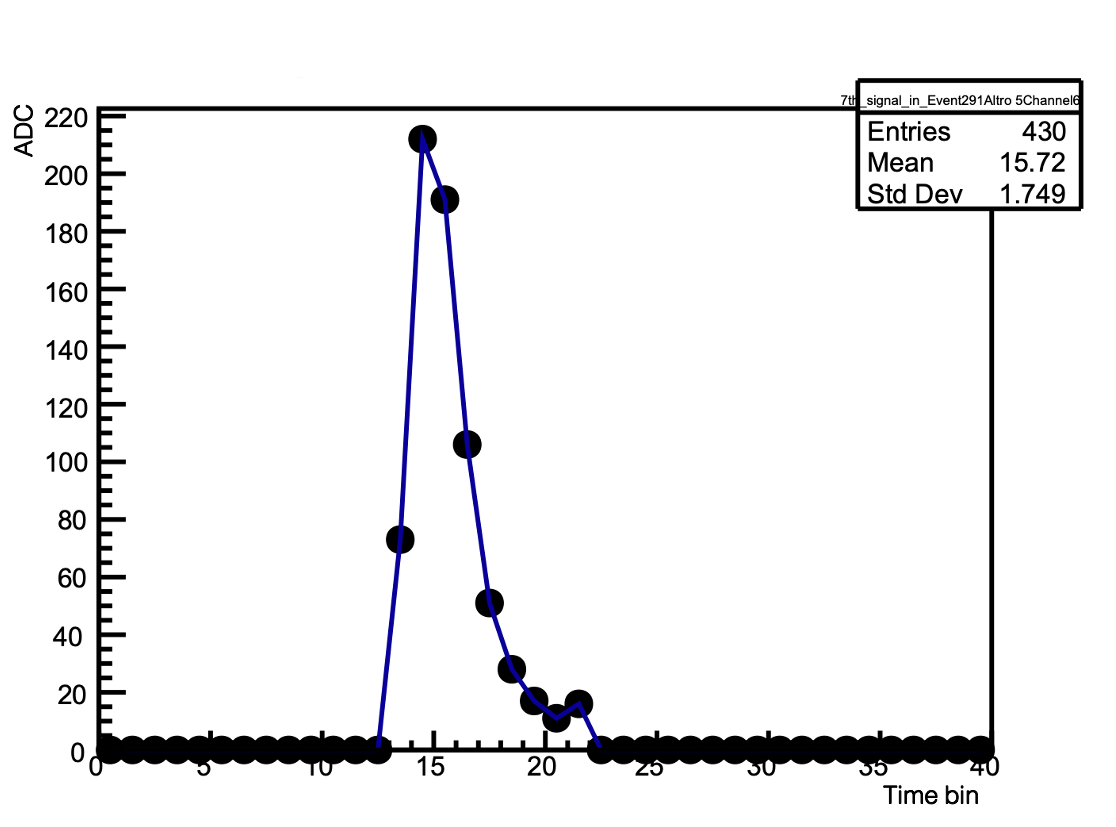
\includegraphics[width=0.7\textwidth,clip]{figures/Chapter3/TPXChannel.png}
    \end{center}
    \caption[TPX电子学单个channel信号读出分布]{TPX电子学单个channel信号读出分布,横轴为time bin,每个time bin时间长度为25ns。纵轴为对应time bin读出的ADC的值}
    \label{fig:TPXChannel}
\end{figure}
整个探测器的触发使用三块闪烁体作为触发系统。触发系统的设置如图\ref{fig:sTGC_Trigger_CR}所示。两个小闪烁体(8cm $*$ 16cm)紧贴探测器放置在小原型机的上下两侧,另一块较大的闪烁体(23cm $*$ 51cm)放置在探测器测试所用平台的下方,三个闪烁体末端接光电倍增管并且通过信号线将其连入信号甄别器,再联入符合单元。当宇宙线穿过闪烁体产生信号被光电倍增管收集到并传入信号甄别器以后,信号甄别器将其转换成负电压的方波信号。每个闪烁体的信号在经过信号甄别器后再被引入符合单元当中,当三个经过信号甄别器的信号被同时引入符合单元的时候符合单元输出一个信号进入trigger board当中,触发探测器电子学采集信号。在此设置之下宇宙线的触发频率大约为30 event/min。
\begin{figure}[htb]
    \begin{center}
    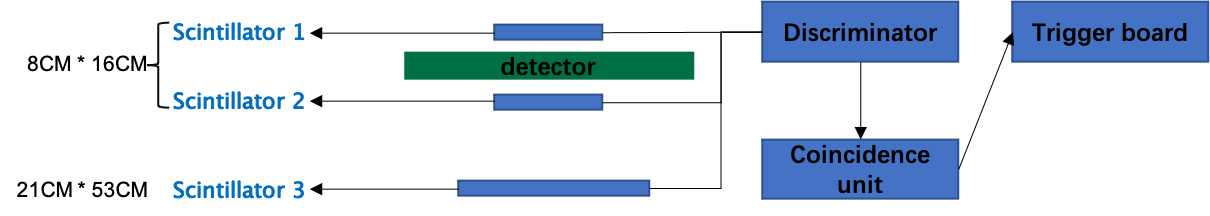
\includegraphics[width=0.7\textwidth,clip]{figures/Chapter3/TiggerCarton.png}
    \end{center}
    \caption[sTGC BNL超净室测试触发系统设置示意图]{sTGC BNL超净室测试触发系统设置示意图}
    \label{fig:sTGC_Trigger_CR}
\end{figure}

在2019年6月之前的测试当中,工作气体为C10,两个室高压均为1425V。在前期测试当中,首先利用丝端读出来验证是否探测器是否可以成功地采集信号。当可以通过丝端读出宇宙线的脉冲信号之后,整个探测器和电子学被接入到数据采集系统(Data Acquisition system, DAQ)当中进行取数。原始的.sfs文件经过解码后得到STAR标准的.daq文件,再通过STAR库中的bfc.C和StRoot中与sTGC相关的maker保存成为常用的ROOT文件格式。

在得到数据之后首先要完成的是数据中的通道和探测器当中实际的每个读出条的对应工作,即map的编写。在山大的小原型机测试中此工作已经完成,只需要将整理得到的文件写成头文件整合到z相关的maker当中去即可。对于19年测试使用的TPX电子学,每个前端电子学板(Front End Electronic Card, FEE Card)上共有两个ALTRO芯片,每个ALTRO芯片上共有16个通道(Channel),每个通道和一个读出条相连接。而不同的前端电子学板上的ALTRO芯片读出时的编号随着前端电子学板的编号变化而变化,这样我们就可以根据电子学读出时的ALTRO芯片编号和通道编号得到唯一对应的读出条编号。示意图见\ref{fig:TPX_map}。从而确定每个信号对应的空间位置来进行之后的效率分析。同时在大原型机和最后的前向窄隙室经济探测器中cluster的重建也需要map,因为后期sTGC的电子学更换为VMM电子学,所以map的对应方式也发生了一些改变。在之后会进行介绍。
\begin{figure}[htb]
    \begin{center}
    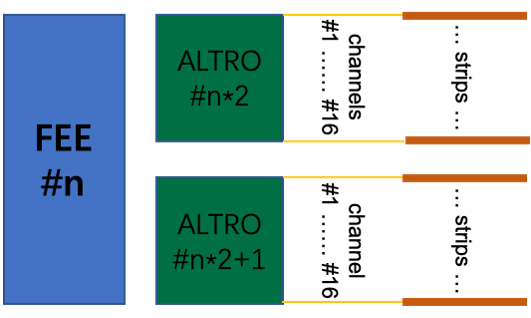
\includegraphics[width=0.7\textwidth,clip]{figures/Chapter3/TPX_map.png}
    \end{center}
    \caption[sTGC TPX电子学与读出条对应示意图]{sTGC TPX电子学与读出条对应示意图}
    \label{fig:TPX_map}
\end{figure}

当电子学正确设置并且可以读出信号之后,接下来的任务就是信号挑选和测试小原型机在C10气体下的效率表现。当工作气体为C10的时候,工作高压在1450V附近,当继续加高电压的时候会发生打火现象影响测试。

首先需要确定探测器的噪声水平,即当电子学接入探测器但探测器高压为0V时电子学可以读到的ADC分布。在此种情况下读到的ADC即为整个探测器和电子学在空负载情况下的噪声水平。因为需要接收宇宙线信号,整个小原型机水平放置,很自然地两个窄隙室被分别称为 top chamber 和 bottom chamber。两个窄隙室在0V下的噪音水平如图\ref{fig:ADC_Distribution_0V}所示。top chamber 和 bottom chamber的噪音水平分别为15ADC 和 20ADC。这两个噪音水平将会作为pedestal参与分析。但在2019年6月最开始的数据分析当中,为了对探测器效率有初步概念,pedestal取得相对较为宽松,两个室均为10ADC。
\begin{figure}[htb]
    \begin{center}
    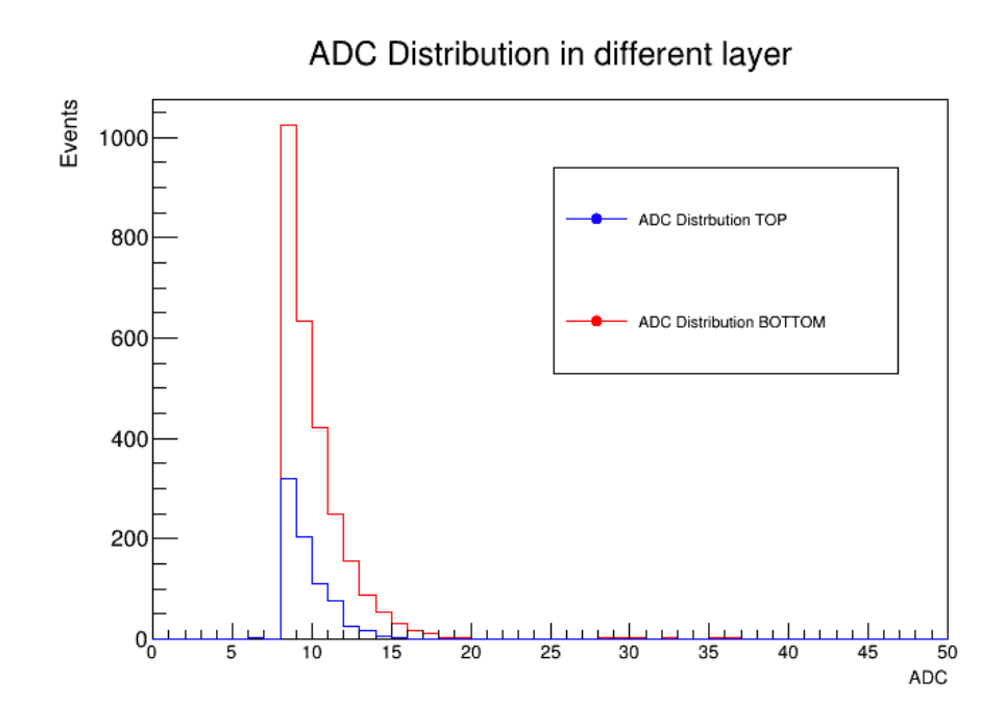
\includegraphics[width=0.7\textwidth,clip]{figures/Chapter3/ADC_Distribution_0V.png}
    \end{center}
    \caption[0V和C10气体下小原型机ADC分布]{0V和C10气体下小原型机ADC分布,蓝色直方图为top chamber的ADC分布,红色直方图为bottom chamber的ADC分布}
    \label{fig:ADC_Distribution_0V}
\end{figure}

当map正确工作后对于每一个事例我们就可以得到这样的一个三维分布:x轴和y轴分别为读出条编号和time bin,z轴为每个读出条在该time bin当中的ADC对应的值。一个事例当中的三维分布如图\ref{fig:Signal_3D}所示。可以看到当加上高压的时候和不加高压相比,信号持续时间和信号的宽度明显的变宽,在初步的分析当中对于信号的宽度和持续时间我们设置了如下的信号判选条件:
\begin{itemize}
    \item 对于单个读出条要求连续的ADC > pedestal的time bin个数大于3。此时认为该读出条有信号响应。
    \item 对于有信号响应的读出条,当相邻的有信号响应的读出条的个数大于3根的时候认为有一个宇宙线事例。
\end{itemize}
\begin{figure}[htb]
    \centering
    \begin{subfigure}[b]{0.45\textwidth}
        \centering
        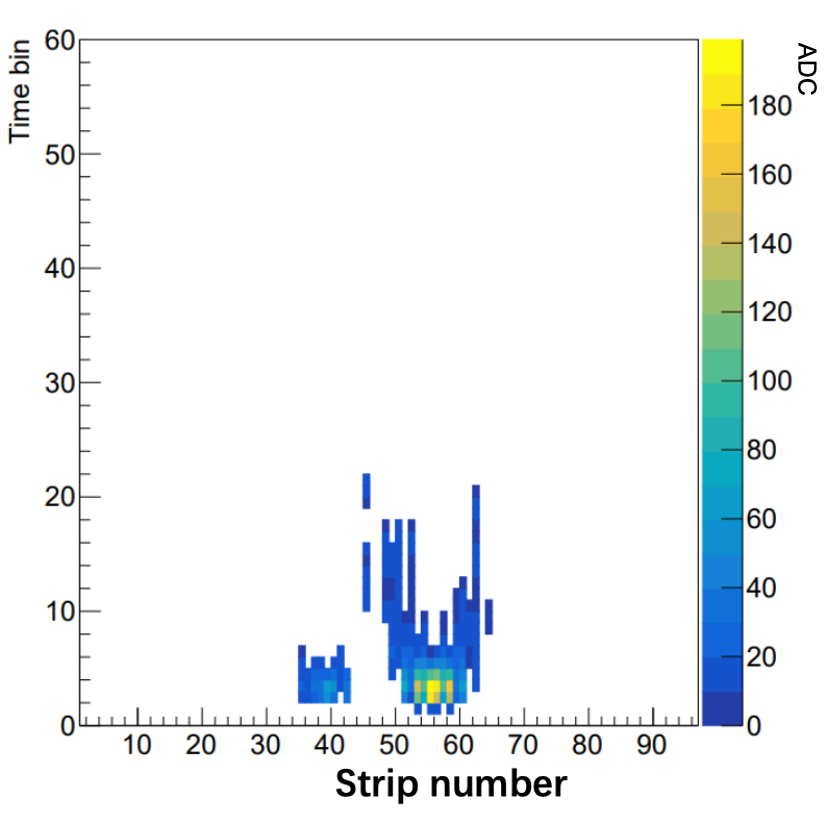
\includegraphics[width=\textwidth,clip]{figures/Chapter3/Strip_TB_ADC.png}
        \caption{1450V}
        \label{fig:Strip_TB_ADC}
    \end{subfigure}
    \hfill
    \begin{subfigure}[b]{0.45\textwidth}
        \centering
        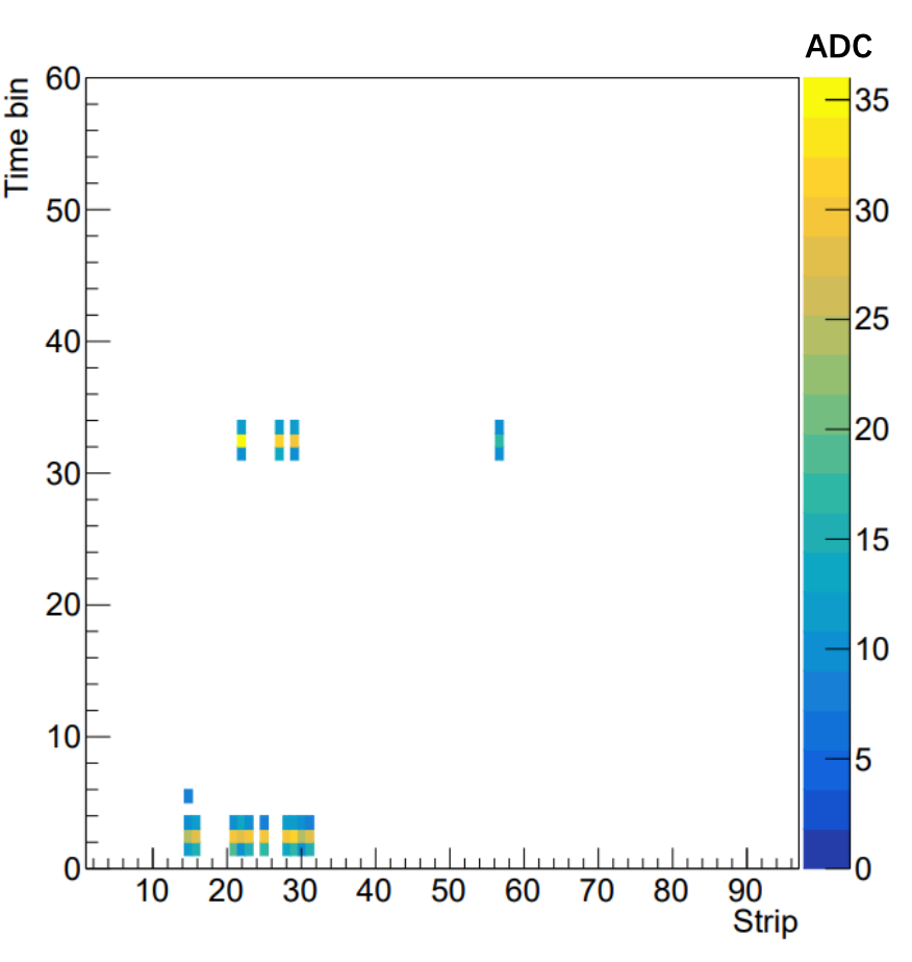
\includegraphics[width=\textwidth,clip]{figures/Chapter3/Strip_TB_ADC_noise.png}
        \caption{0V}
        \label{fig:Strip_TB_ADC_noise}
    \end{subfigure}
    \caption[一个事例当中每个读出条上ADC随time bin 分布示意图]{\ref{fig:Strip_TB_ADC}为bottom chamber在高压为1450V下一个信号事例。\ref{fig:Strip_TB_ADC_noise}为bottom chamber在高压为0V下的一个噪音事例。}
       \label{fig:Signal_3D}
\end{figure}
其中根据测试环境的变化pedestal的值可能发生变化,在首次测试当中pedestal取10,top chamber和bottom chamber的高压分别为1450V和1350V。在此设置下,根据这样的宇宙线事例挑选条件我们对在超净室取得的第一个run进行了分析,结果如图\ref{fig:Cosmic_first}所示。对于效率的计算分别采取了以下两种计算方式:
\begin{itemize}
    \item 宇宙线触发。
    \\效率计算公式如下:$\epsilon_{top(bottom)~chamber} = N_{top(bottom)~chamber}/N_{cosmic~event}$
    \item 窄隙室相互触发。
    \\效率计算公式如下:$\epsilon_{top(bottom)~chamber} = N_{two~chambers}/N_{bottom(top)~chamber}$
\end{itemize}
其中$N_{cosmic~event}$为总的宇宙线触发事例数,$N_{top(bottom)~chamber}$为一个事例当中top(bottom) chamber有信号响应的事例数,$N_{two~chambers}$为一个事例当中top和bottom chmaber同时有信号响应的事例数。在这个run当中的各种计算方式下的效率如表\ref{tab:Cosmic_first}所示:
\begin{table}[h!]
    \centering
    \caption{小原型机BNL本地测试第一个宇宙线run效率测试结果}
    \label{tab:Cosmic_first}
    \begin{tabularx}{0.9\textwidth} {| >{\centering\arraybackslash}X |>{\centering\arraybackslash}X |>{\centering\arraybackslash}X |>{\centering\arraybackslash}X |}
        \hline
         &高压& 宇宙线触发 & 窄隙室相互触发\\
        \hline
        top chamber & 1450V & 2.5\% & 17.5\%\\
        \hline
        bottom chamber& 1350V & 0.4\% & 2.7\% \\
        \hline
    \end{tabularx}
\end{table}
\begin{figure}[htb]
    \begin{center}
    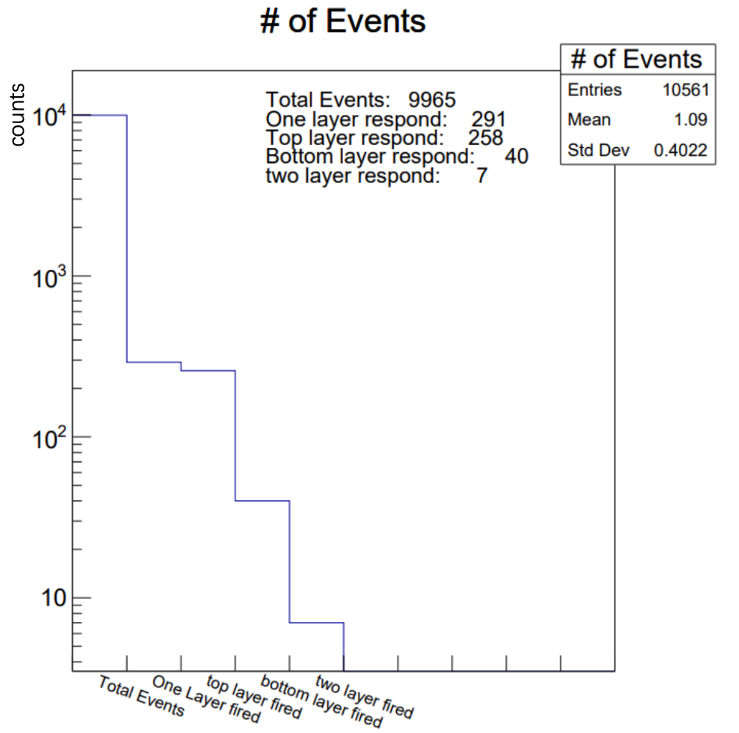
\includegraphics[width=0.7\textwidth,clip]{figures/Chapter3/Cosmic_first.png}
    \end{center}
    \caption[小原型机第一个宇宙线run的测试结果]{小原型机第一个宇宙线run的测试结果,其中total events 为总的触发事例数,one layer fired 为在一个事例当中top 或者 bottom chamber有信号的事例数,top layer fired和bottom layer fired分别为一个事例中top和bottom chamber有信号的事例数,two layers fired为一个事例中两个chamber同时能找到信号的事例数。}
    \label{fig:Cosmic_first}
\end{figure}
可以看到初步测试的结果显示在使用C10气体作为工作气体的情况下整个探测器的探测效率很低,无法满足正常的使用需求。在2019年9月,STAR获得了在超净室当中使用正戊烷的许可,对C10和正戊烷两种工作气体下的探测器表现进行了进一步的研究。

首先测试的是在相同高压下对两种不同的工作气体的流速对探测效率的影响。在不同工作气体工况下保持高压不变,在气体流速为80 cc/min 和 200 cc/min下进行测试。C10气体下两个chamber的高压均设置为1425V,正戊烷为工作气体时两个chamber高压均为2800V。信号挑选的判选条件如表\ref{tab:Cosmic_gasflow}所示
\begin{table}[h!]
    \centering
    \caption{气体流速测试宇宙线信号挑选判选条件}
    \label{tab:Cosmic_gasflow}
    \begin{tabularx}{0.9\textwidth} {| >{\centering\arraybackslash}X |>{\centering\arraybackslash}X |>{\centering\arraybackslash}X |>{\centering\arraybackslash}X |>{\centering\arraybackslash}X |}
        \hline
         & timming &ADC pedestal& 单信号条信号持续时间 & 信号宽度\\
        \hline
        C10 & 0-30 time bin & 10 ADC & >3 time bin & > 3 strips\\
        \hline
        ${\rm CO_2}$ + n-Pentane& 0-30 time bin & 10 ADC & >3 time bin & > 3 strips\\
        \hline
    \end{tabularx}
\end{table}
在不同流速下的效率测试结果显示不论是C10还是正戊烷作为工作气体,探测器的效率都没有发生明显的改变,结果如图\ref{fig:GasFlow}所示。证明探测器可以在不同的气体流速下稳定工作。同时可以看到,当正戊烷作为工作气体的时候探测器可以达到很高的探测效率,99约\%,符合探测器设计时的高效率的要求。
\begin{figure}[htb]
    \begin{center}
    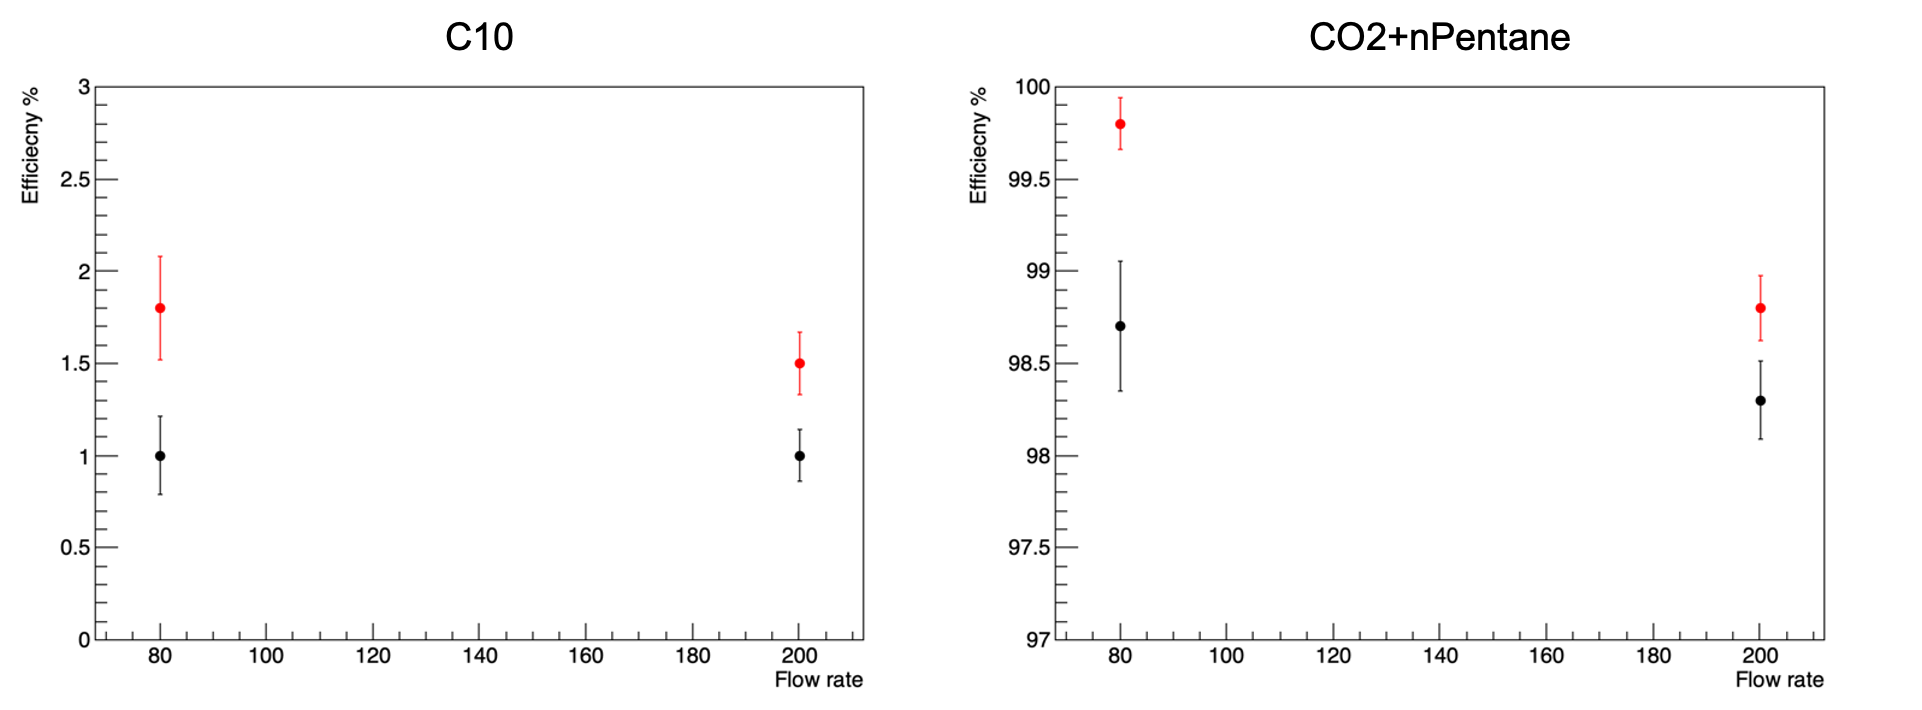
\includegraphics[width=0.9\textwidth,clip]{figures/Chapter3/GasFlow.png}
    \end{center}
    \caption[小原型机不同气体不同流速效率测试结果]{小原型机不同气体不同流速效率测试结果。左图工作气体为C10气体,右图工作气体为${\rm CO_2}$ + n-Pentane}
    \label{fig:GasFlow}
\end{figure}

根据参考文献[],在相同的气压下正戊烷的在混合气体当中所占的百分比和温度正相关,因为气体混合系统并不是完美的混合系统,气体的温度或者组分会在一定范围内浮动,所以我们也需要测试当正戊烷在不同的温度情况下的探测效率表现。测试时气体流速固定均为80 cc/min,信号判选条件以及高压和流速测试时判选条件相同。测试结果如图\ref{fig:Temperature}所示。可以看到当温度在${\rm 15^{\circ}C}$ 至 ${\rm 19^{\circ}C}$的范围内浮动时整个探测器都可以保持很高的探测效率,工作状况稳定,在目标的温度范围内探测器可以稳定工作。
\begin{figure}[htb]
    \begin{center}
    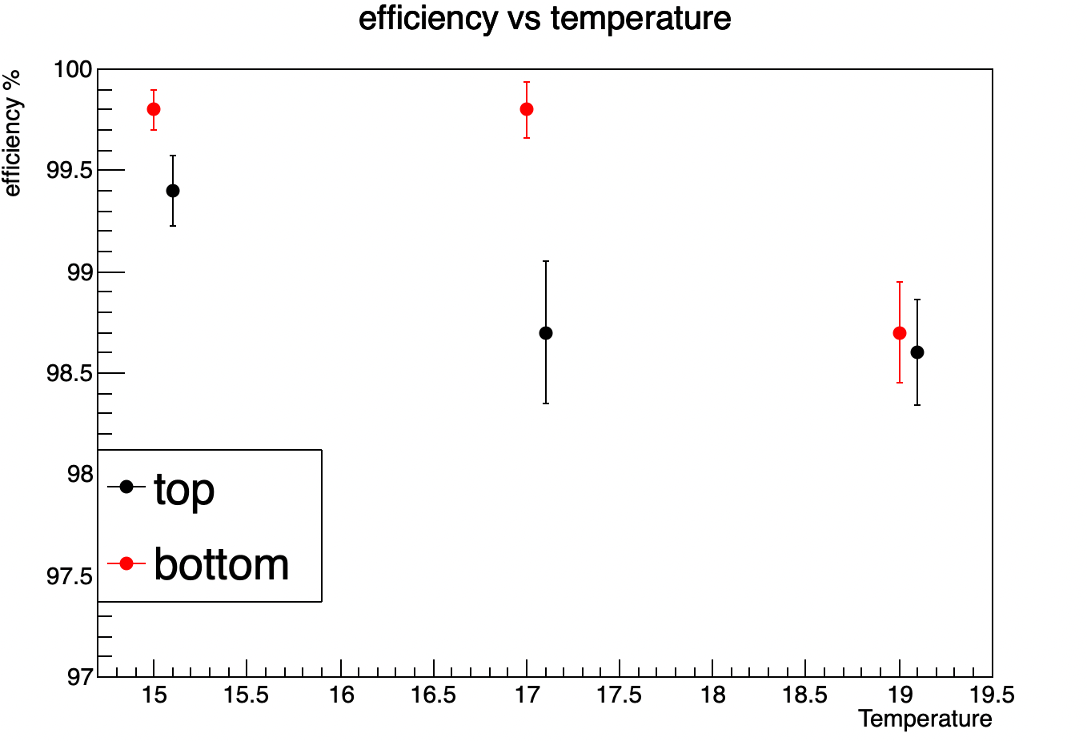
\includegraphics[width=0.75\textwidth,clip]{figures/Chapter3/Temperature.png}
    \end{center}
    \caption[小原型机正戊烷工作气体下不同温度效率测试结果]{小原型机正戊烷工作提起不同温度效率测试结果,黑色圆点为top chamber结果,红色圆点为bottom chamber结果}
    \label{fig:Temperature}
\end{figure}

除了对C10和正戊烷作为工作气体进行测试以外,我们还尝试了对其他几种工作气体进行测试,试图找出可以替代正戊烷的工作气体以避免因为正戊烷的可燃性而带来的工程以及安全问题。但经过了几组不同的工作气体测试后发现除了正戊烷以外其余的工作气体均无法达到预期的探测效率,结果如表\ref{tab:CR_DifferentGas}所示。
\begin{table}[h!]
    \centering
    \caption{不同工作气体小原型机效率测试结果}
    \label{tab:CR_DifferentGas}
    \begin{tabularx}{0.95\textwidth} {| >{\centering\arraybackslash}X |>{\centering\arraybackslash}X |>{\centering\arraybackslash}X |>{\centering\arraybackslash}X |}
        \hline
         & 工作气体 & 高压 & 效率 \\
        \hline
        top chamber & Ar+${\rm CO_2}$+${\rm CH_4}$ & 2200 V & 6.2\%  \\
        \hline
        bottom chamber& Ar+${\rm CO_2}$+${\rm CH_4}$ & 2200 V& 2.5\% \\
        \hline
        top chamber & Ar+${\rm CO_2}$+${\rm CH_4}$ & 2300 V & 10.3\%  \\
        \hline
        bottom chamber& Ar+${\rm CO_2}$+${\rm CH_4}$ & 2300 V& 3.3\% \\
        \hline
        top chamber & Ar+${\rm CO_2}$+异丁烷 & 2200 V & 5.8\%  \\
        \hline
        bottom chamber& Ar+${\rm CO_2}$+异丁烷& 2200 V& 2.3\% \\
        \hline
    \end{tabularx}
\end{table}

\subsubsection{束流测试}

在第一次超净室测试验证了TPX电子学可以正常的在小原型机上工作并且取数以后,于2019年6月小原型机被安装在了STAR的西侧进行取数测试其在束流环境下的表现。触发使用STAR minimum bias(MiniBias, MB) trigger。但在2019年的run当中,MB trigger 并不是专门为前向的探测设计的trigger,无法通过trigger的数目来作为效率测试的分母。所以对于效率的测试只能使用互相触发的方式来进行。

在小原型机的束流测试中,我们对探测器进行了高压扫描。同样因为安全许可问题,在2019年的束流测试中只能使用C10作为工作气体。首先在高压为0 V时进行取数来确定pedestal,单信号条信号持续时间,信号宽度等判选条件的取值。束流测试当中的信号判选条件设置如表\ref{tab:Beam_HVScan}所示:
\begin{table}[h!]
    \centering
    \caption{束流测试中高压扫描信号判选条件}
    \label{tab:Beam_HVScan}
    \begin{tabularx}{0.95\textwidth} {| >{\centering\arraybackslash}X |>{\centering\arraybackslash}X |>{\centering\arraybackslash}X |>{\centering\arraybackslash}X |>{\centering\arraybackslash}X |}
        \hline
         & timming &ADC pedestal& 单信号条信号持续时间 & 信号宽度\\
        \hline
        top chamber & < 10 time bin & 10 ADC & >3 time bin & > 3 strips\\
        \hline
        bottom chamber& < 10 time bin & 10 ADC & >3 time bin & > 3 strips\\
        \hline
    \end{tabularx}
\end{table}
高压扫描从1400 V开始,每隔25 V取数。当电压升到1500 V的时候探测器频繁出现打火问题,所以电压扫描到此为止。除了高压以外剩下的所有触发以及气体的设置均不变。探测器互相触发所测量到的效率如图\ref{fig:BeamHV}所示。在C10工作气体下探测器的工作效率随着高压的增加呈线性增加,但是仍然无法达到探测器设计时的效率要求。且因为最后的设计是多层sTGC作为整个径迹探测系统,如果单层只有25\%左右的探测效率,最后四层合并对于单条径迹的探测效率期望只有0.3\%,完全无法接受。所以C10作为工作气体的想法经过束流测试之后被完全否决。综合之前的不同气体组分的测试结果,正戊烷被最后确定为前向小读出条窄隙室径迹探测器的工作气体。
\begin{figure}[htb]
    \begin{center}
    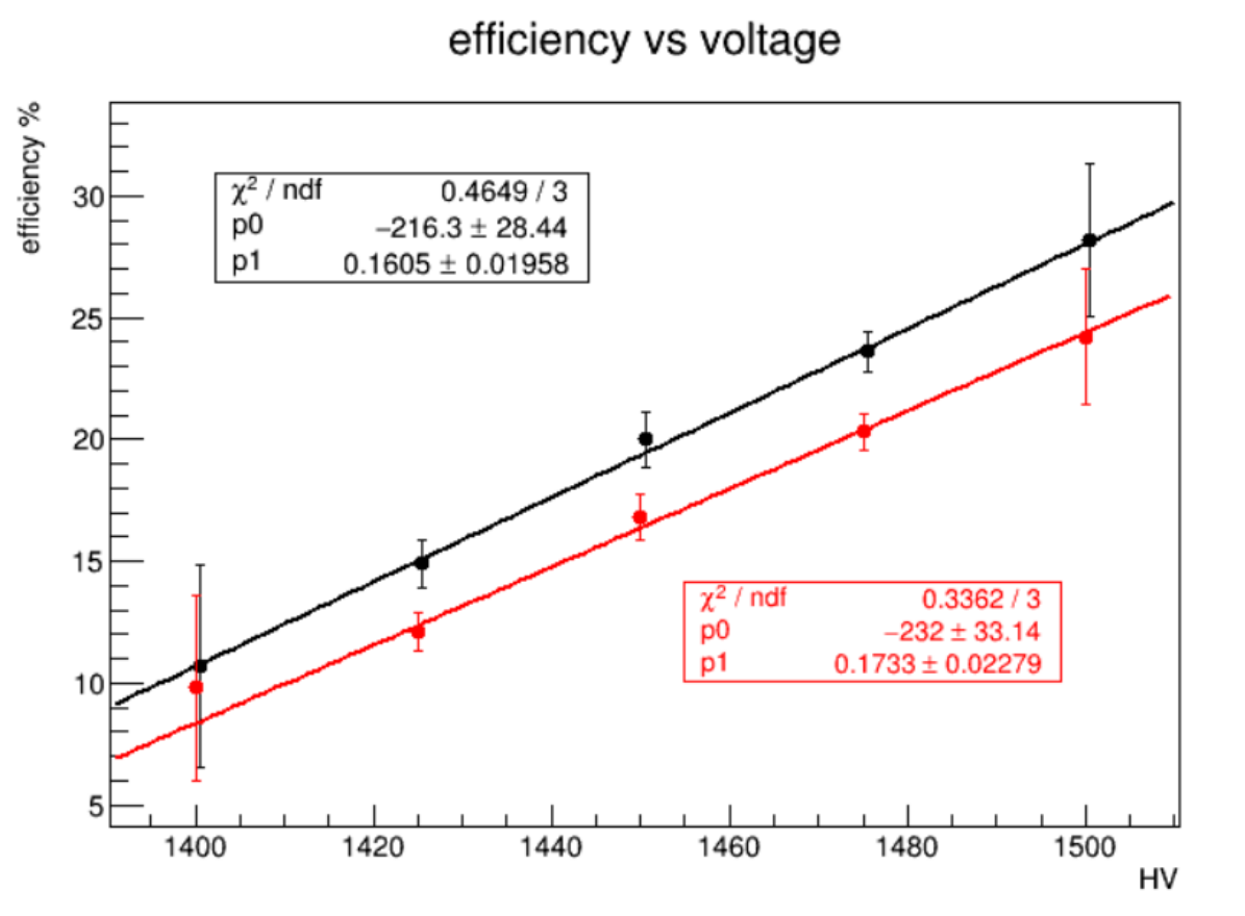
\includegraphics[width=0.75\textwidth,clip]{figures/Chapter3/BeamHVpng.png}
    \end{center}
    \caption[小原型机C10工作气体下束流环境中不同高压效率测试结果]{小原型机C10工作气体下束流环境中不同高压效率测试结果,黑色圆点为top chamber结果,红色圆点为bottom chamber结果。error bar 仅显示统计误差,和数据量直接相关,在1400V时因为探测效率很低、在1500V因为经常发生打火探测器停止工作所以数据量明显小于其他能量。}
    \label{fig:BeamHV}
\end{figure}